%-----------------------------------------------------------------------------%
\chapter{ANALISIS DAN PERANCANGAN SISTEM}

%-----------------------------------------------------------------------------%

%
\vspace{4.5pt}

Bab ini akan membahas tentang proses bisnis dan arsitektur dari rumah sakit Apertura. Lalu akan membahas analisa terkait proses bisnis dan arsitektur yang baru untuk diterapkan pada aplikasi, termasuk segala komponen penyusun sistem yang baru mulai dari database, \textit{tools}, IDE (\textit{Integrated Development Environment}), \textit{framework} yang digunakan dalam membangun aplikasi. Selanjutnya akan dibahas mengenai perancangan \textit{service} dengan menggunakan konsep REST dan pembuatan API dari \textit{service} tersebut.
\section{Arsitektur Monolitik pada Software Apertura}
Menurut Sam Newman, terdapat 2 parameter yang membedakan arsitektur monolitik dengan microservice, pertama adalah tingkat \textit{coupling} dan yang kedua adalah tingkat \textit{cohesion} dari aplikasi tersebut. Pernyataan ini kemudian didukung oleh Chris Richardson yang menjelaskan bahwa kedua parameter ini dapat ditinjau dari berbagai sisi yang membentuk aplikasi tersebut, antara lain: data menejemen, cara berkomunikasi, dan metode \textit{deployment} sebuah aplikasi.

\begin{enumerate}[leftmargin=*]
	\item \textbf{Data manajemen.} Aplikasi Apertura menerapkan model tersentralisasi yang sangat besar. Kurang lebih terdapat 120 tabel yang terdapat dalam 1 buah database tunggal. Namun semakin banyak model shared database yang digunakan, maka semakin tinggi pula derajat \textit{coupling} aplikasi tersebut, dan tingginya derajat \textit{coupling} merupakan salah satu ciri dari monolitik.
	\item \textbf{Cara berkomunikasi.} Modul dalam database Apertura dapat mengakses langsung tabel milik modul lain dengan melakukan \textit{querry} terhadap tabel tersebut. Cara berkomunikasi seperti ini seperti ini menjadi ciri dari arsitektur monolitik.
	\item \textbf{Bentuk deployment.} Tabel-tabel dan database Apertura disimpan dalam 1 buah database server yang sama. Penempatan server terpusat ini dianggap kurang menunjang konsep \textit{high availability} apabila terjadi masalah pada server. Aplikasi menjadi sangat tergantung dengan server tunggal tersebut dan menjadi ciri derajat \textit{coupling} yang tinggi.
\end{enumerate}
\newpage
Berdasarkan analisis dari ketiga faktor diatas, maka dapat disimpulkan bahwa arsitektur dari aplikasi Apertura adalah monolitik.\\
Arsitektur monolitik Apertura dapat digambarkan dengan deployment diagram dibawah:

\begin{adjustbox}{width=1\textwidth}
\begin{minipage}{\linewidth}
	\framebox[\textwidth]{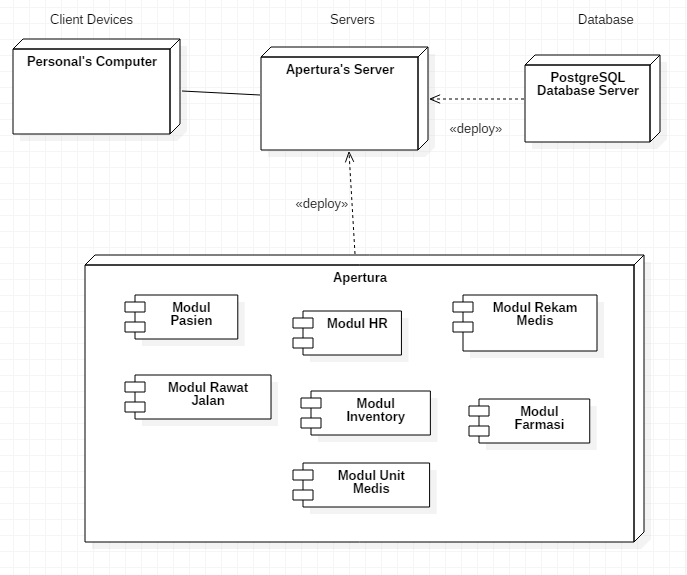
\includegraphics[width=10cm]{images/deployment_diagram.png}}	
	\captionof{figure}{Pemodelan Software Apertura dengan deployment diagram.}
\end{minipage}
\end{adjustbox}

\section{Tinjauan Umum Proses Bisnis Pelayanan Rawat Jalan}
Proses bisnis dalam rumah sakit Apertura melibatkan beberapa modul yang saling berinteraksi, modul-modul tersebut terdiri dari bagian yang lebih kecil lagi. Analisis berdasarkan proses bisnis berdasarkan kegunaannya akan lebih mudah untuk menentukan service yang akan terbentuk nantinya.\\
Modul-modul dari aplikasi Apertura antara lain: modul pasien, modul HR (human resources) yang meliputi data dokter, bidan, dan perawat, modul rekam medis, modul farmasi, modul inventori, modul akunting dan finansial, modul invoicing  dan pembayaran, modul rawat jalan, modul rawat inap, modul pemeriksaan penunjang, dan modul integrasi SEP (Surat Eligibilitas Pasien) BPJS.

Dari semua modul tersebut, penulis akan mengambil contoh kasus rawat jalan. Rawat jalan adalah tindakan perawatan pasien yang tidak menginap. Pasien yang datang akan mendaftar ke unit rawat jalan dan dicek apakah pasien tersebut terdaftar di BPJS, kemudian berdasarkan masalah pasien, pasien akan dirujuk ke unit medis yang ada di rumah sakit. Unit medis dari rumah sakit terdiri dari unit medis spesialis anak, spesialis jantung, dan spesialis penyakit dalam. Tiap unit medis memiliki satu atau lebih dokter spesialis dari bidang unit medis tersebut. Pasien kemudian akan ditangani oleh dokter yang bertugas di unit medis tersebut. Proses penanganan pasien dimulai dari konsultasi keluhan, pemeriksaan penunjang, dan diagnosis penyakit.

Hasil dari pemeriksaan tersebut akan disimpan dalam rekam medis pasien di rumah sakit. Modul rawat jalan akan mengeluarkan resep obat yang dapat pasien ambil di farmasi. Modul rawat jalan juga akan mengeluarkan detail faktur yang dibutuhkan untuk proses pembayaran. 

Maka dari itu, modul rawat jalan akan melibatkan modul pasien, HR, unit medis, farmasi, rekam medis, pemeriksa penunjang, pembayaran dan penagihan, integrasi BPJS, dan modul rawat jalan itu sendiri.\\
Berikut adalah penggambaran proses bisnis dari pelayanan rawat jalan:

\begin{adjustbox}{width=1\textwidth}
	\begin{minipage}{\linewidth}
		\framebox[\textwidth]{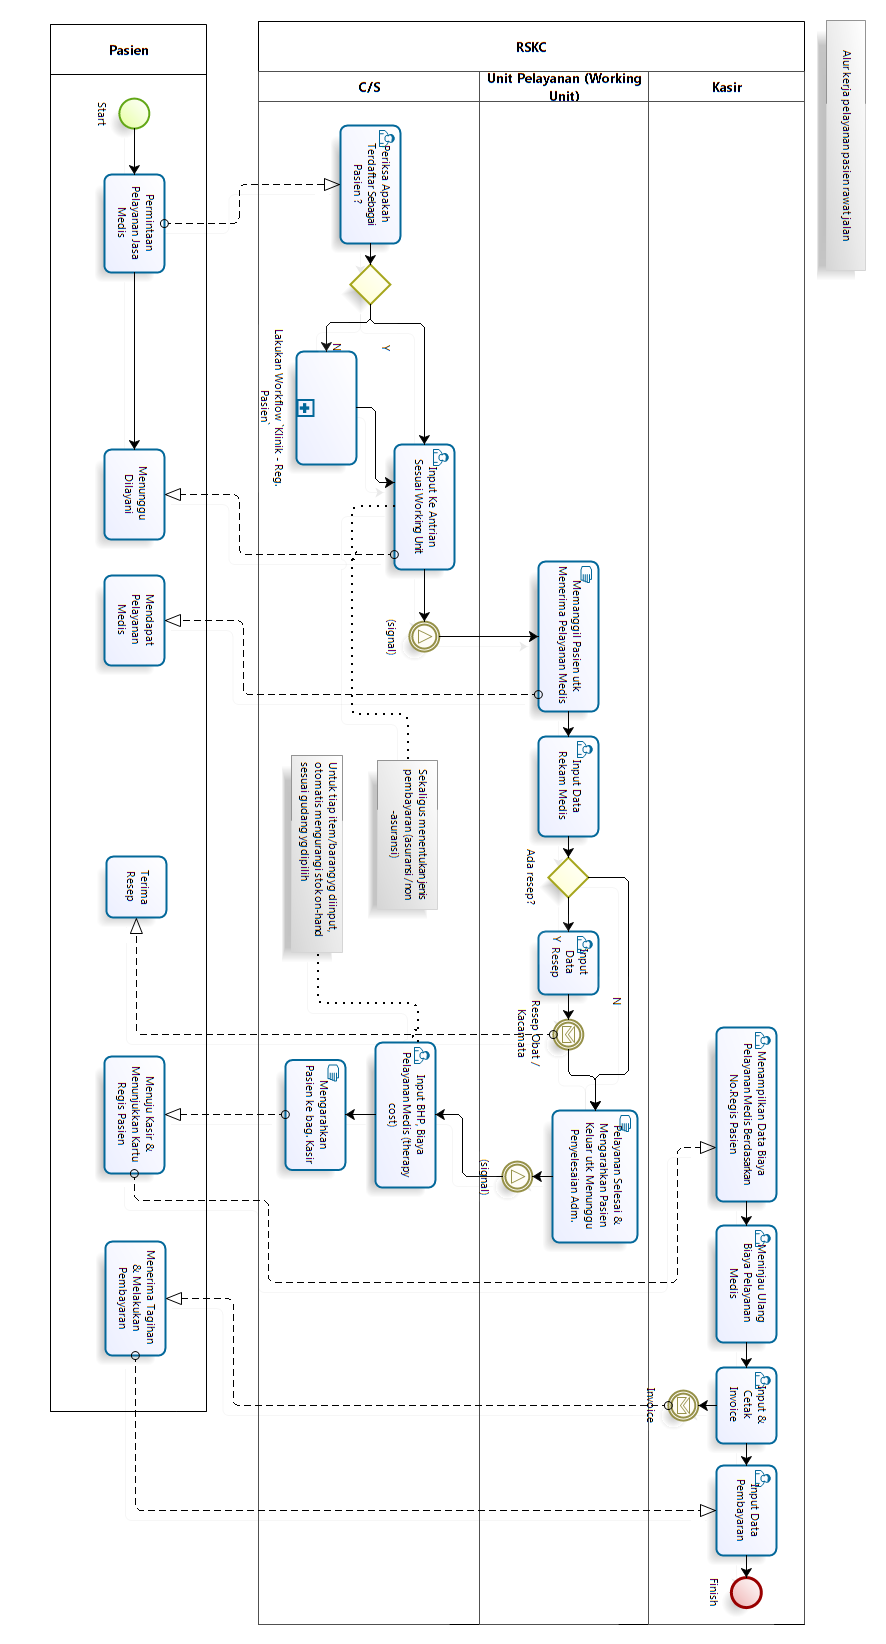
\includegraphics[width=12cm]{images/workflow_proccess.png}}	
		\captionof{figure}{Proses bisnis rawat jalan.}
	\end{minipage}
\end{adjustbox}

\section{Pembahasan Modul dan Kelas Penyusun}
Pada bagian ini akan dijelaskan fungsi dan kelas-kelas dari setiap modul dalam kaitannya dengan proses bisnis di rumah sakit.

\begin{enumerate}[leftmargin=*]
	\item \textbf{Modul Pasien.} Modul pasien berfungsi untuk menyimpan, memperbaharui, pencarian, dan menampilkan data pasien. Data pasien juga meliputi detail lengkap dari data keluarga atau kerabat yang menjadi penanggung jawab pasien. Kelas dari modul pasien adalah pasien itu sendiri.
	\item \textbf{Modul \textit{Human Resource}.} \textit{Human Resource} adalah modul yang mengelola semua pengguna dan pegawai dalam rumah sakit, modul ini dapat disebut juga sebagai modul karyawan. Beberapa contoh yang termasuk dalam modul ini adalah dokter, bidan, dan perawat. Modul ini menjadi modul dasar yang dibutuhkan modul lain, karena terkait pencatatan pengguna yang melakukan input data. Kelas-kelas dari modul ini meliputi dokter, bidan, dan perawat. Namun dalam contoh kasus rawat jalan yang akan diangkat, kelas yang diambil hanya dokter saja.
	\item \textbf{Modul Unit Medis.} Unit medis dari rumah sakit terdiri dari unit medis spesialis anak, spesialis jantung, dan spesialis penyakit dalam. Tiap unit medis memiliki satu atau lebih dokter spesialis dari bidang unit medis tersebut. Pasien akan ditangani oleh dokter yang bertugas di unit medis tersebut.
	\item \textbf{Modul Rawat Jalan.} Rawat jalan adalah pelayanan medis kepada pasien untuk tujuan perawatan tanpa mengharuskan pasien tersebut untuk menginap. Rawat jalan menjadi perantara interaksi dari pasien dengan unit medis, rawat jalan menyimpan data perawatan yang kemudian akan disimpan dalam rekam medis. Hasil dari rawat jalan akan kemudian dibutuhkan oleh bagian pembayaran dan juga farmasi.
\end{enumerate}

Berikut adalah penggambaran relasi dari modul rawat jalan menggunakan komponen diagram:

\begin{adjustbox}{width=1\textwidth}
	\begin{minipage}{\linewidth}
		\framebox[\textwidth]{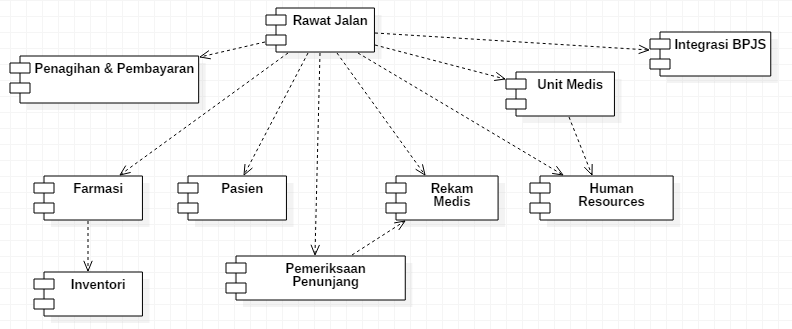
\includegraphics[width=13cm]{images/komponen_diagram_rawatjalan.png}}	
		\captionof{figure}{Komponen diagram rawat jalan.}
	\end{minipage}
\end{adjustbox}

\section{Identifikasi Teknologi yang Digunakan pada Aplikasi Apertura}
Saat ini teknologi aplikasi yang digunakan Rumah Sakit Apertura menggunakan arsitektur monolitik dengan database yang tersentralisasi pada 1 buah server. Database Apertura sendiri menggunakan PostgreSQL 9. PostgreSQL merupakan salah satu object-relational database management system (ORDMS) yang tersedia secara \textit{open source}. Database Apertura terdiri dari kurang lebih 120 tabel yang saling berelasi. Cara pertukaran data yang digunakan oleh Apertura saat ini adalah query \textit{database} langsung dan database dibuat \textit{shared} sehingga semua modul bisa mengakses \textit{database} secara bebas.
Aplikasi Apertura digunakan oleh beberapa kelompok pengguna, antara lain bagian kasir rumah sakit, registrasi rawat jalan, registrasi rawat inap, kasir apotik, kasir rawat jalan, dokter, staf administrasi umum, staf keuangan, staf rekam medis, staf administrasi BPJS. Dalam setiap harinya terjadi rata-rata 400 pendaftaran rawat jalan yang ditangani oleh kurang lebih 30 dokter yang bertugas.
Platform yang diimplementasi oleh Apertura adalah bentuk aplikasi desktop. \textit{User interface} yang ditampilkan dalam aplikasi tidak terpisah secara moduler, melainkan satu kesatuan aplikasi besar yang kemudian dipisahkan berdasarkan kebutuhan user yang menggunakan aplikasi.

\subsection{Peluang dan Antisipasi Pengembangan Sistem}
Berdasarkan analisis yang dilakukan, peluang pengembangan sistem baru yang diusulkan dalam penelitian kali ini melihat 3 faktor utama, yaitu faktor data, platform, dan kelincahan proses kerja. Adapun peluang pengembangan tersebut dijelaskan pada point di bawah :

\begin{enumerate}[leftmargin=*]
	\item Desain arsitektur yang baru dibuat lebih moduler dan terpisah, dengan menjadikan setiap layanan menjadi service mandiri dapat mengurangi tingkat \textit{coupling} yang terlalu tinggi yang dapat menyebabkan kendala dalam proses pengembangan sistem. Pada desain microservice, perubahan yang dilakukan dalam sebuah modul tidak perlu diketahui oleh modul lain, menjadikan proses \textit{deployment} lebih lincah dan cepat dari sebelumnya karena tiap tim pengembang sistem dapat bekerja secara mandiri. Selain itu dengan tidak ada data yang disimpan terpusat pada sebuah server, desain microservice juga meningkatkan tingkat keamanan dan \textit{availabilitas} dari keseluruhan sistem.
	\item Desain yang baru disiapkan untuk kebutuhan \textit{cross-platform}, menjadikan sistem lebih lincah dan dapat digunakan di lebih banyak perangkat seperti komputer pribadi dan juga telepon genggam. Dengan siapnya fitur \textit{cross-platform} ini, dapat menjadi peluang agar interaksi dari \textit{user} dapat ditingkatkan, misalnya untuk kebutuhan pendaftaran antrian rawat jalan menggunakan aplikasi di telepon genggam.
	\item Sistem lebih kuat untuk menangani \textit{multiple user} dikarenakan arsitektur microservice memiliki server masing-masing yang bekerja khusus untuk layanannya sendiri, tidak bercampur dengan modul lain.
\end{enumerate}

\section{Perancangan Arsitektur Microservice}
Dengan menggunakan pattern dekomposisi berdasarkan kemampuan bisnisnya, service yang akan terbentuk terdapat 5 buah, yaitu \textit{service Customer}, \textit{Human Resources}, \textit{Medical Unit}, \textit{Medical Records} dan \textit{service Outpatient} (rawat jalan). Modul-modul \textit{service} tersebut didapat dari hasil analisa proses bisnis dalam pelayanan rawat jalan (gambar 3.2). Apabila sebelumnya semua entitas berada dalam satu buah \textit{server} yang sama, kali ini masing-masing service tersebut akan berdiri mandiri di \textit{server} yang berbeda. Perancangan berikut akan menjelaskan migrasi ke arsitektur baru dan menjawab rumusan masalah yang pertama. Berikut adalah analisa perancangan service yang baru.
\subsection{Perancangan Service \textit{Customer}}
Customer merupakan turunan dari \textit{class} Contact yang berisi biodata pasien rumah sakit. Customer bisa dibedakan menjadi 2, yaitu \textit{customer} yang memiliki asuransi dan yang tidak memiliki asuransi. Namun selain Customer, \textit{class} Contact juga digunakan oleh modul \textit{Human Resources} dikarenakan atribut \textit{contact} dapat digunakan untuk \textit{customer} maupun juga \textit{employee}. Ketergantungan dari desain seperti ini dianggap terlalu tinggi dan menyebabkan data \textit{customer} dan \textit{employee} menjadi tercecer dikarenakan ditempatkan dalam satu tabel yang sama.
Desain baru yang diimplementasikan untuk penelitian kali ini adalah memisahkan fungsi \textit{contact} menjadi lebih spesial untuk \textit{customer} dan juga \textit{employee}. Kelebihan dari desan ini adalah tingkat ketergantungan yang lebih rendah dan tingkat \textit{availabilitas} yang lebih tinggi. Maka dalam modul \textit{customer} akan berisi entitas \textit{customer}, \textit{contact}, dan \textit{class} relasi dari kedua entitas tersebut.\\
Berikut adalah rancangan untuk \textit{webservice customer} digambarkan menggunakan \textit{class diagram}

\begin{adjustbox}{width=1\textwidth}
	\begin{minipage}{\linewidth}
		\framebox[\textwidth]{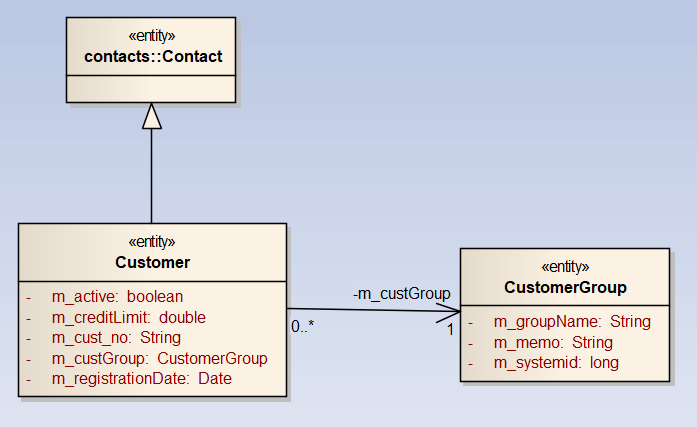
\includegraphics[width=12cm]{images/Customer.png}}	
		\captionof{figure}{Rancangan service \textit{customer}}.
	\end{minipage}
\end{adjustbox}
\subsection{Perancangan Service \textit{Human Resource}}
Modul \textit{Human Resource} berisi data \textit{employee} yang bekerja di rumah sakit. Modul ini pula menjelaskan departemen, dan spesialitas pekerjaan \textit{employee} tersebut di rumah sakit. Sama halnya dengan \textit{customer}, \textit{employee} juga merupakan turunan dari \textit{class contact} yang berdiri mandiri dan terpisah fungsinya dengan yang digunakan untuk \textit{customer}, kelebihan dari desan ini adalah tingkat ketergantungan yang lebih rendah dan tingkat \textit{availabilitas} yang lebih tinggi.\\
Berikut adalah rancangan untuk \textit{webservice human resource} digambarkan menggunakan \textit{class diagram}

\begin{adjustbox}{width=1\textwidth}
	\begin{minipage}{\linewidth}
		\framebox[\textwidth]{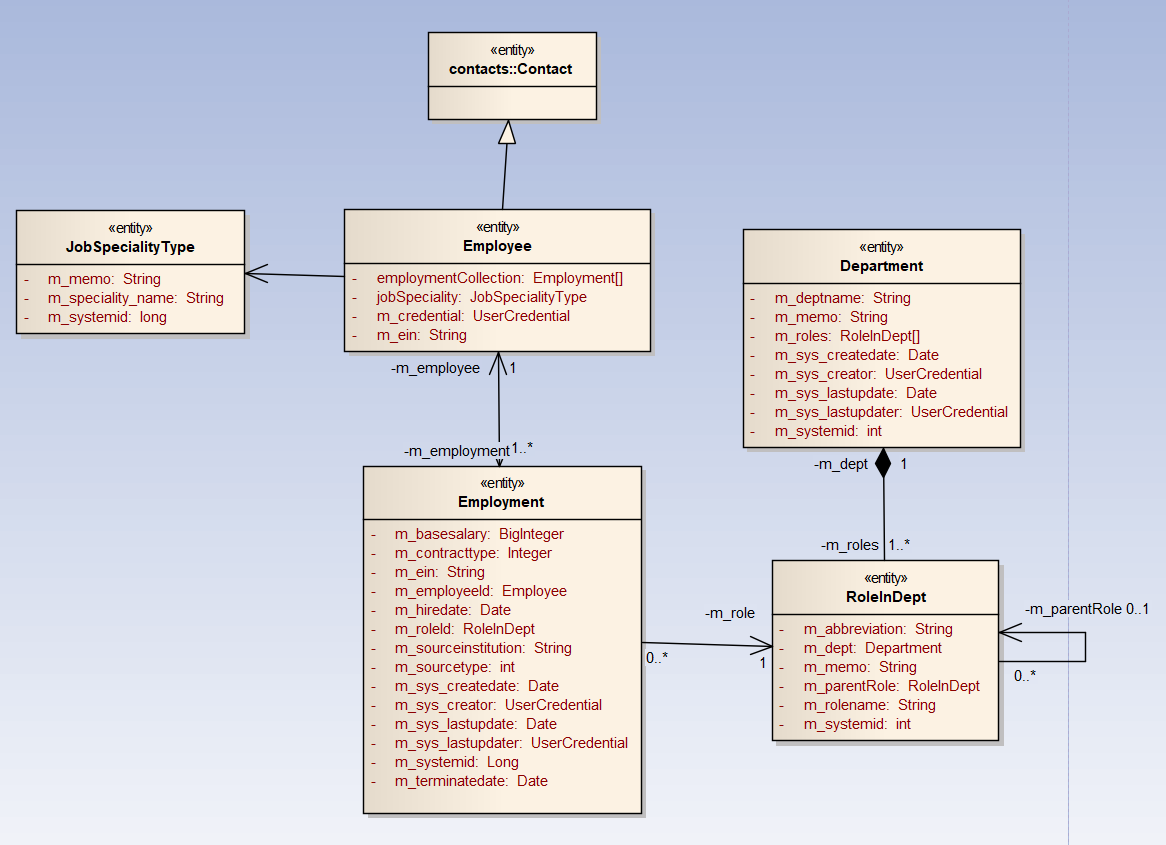
\includegraphics[width=12cm]{images/hr.png}}	
		\captionof{figure}{Rancangan service \textit{human resource}}.
	\end{minipage}
\end{adjustbox}

\subsection{Perancangan Service Unit Medis}
Modul Unit Medis merupakan unit representasi tempat \textit{employee} bekerja, unit medis sendiri adalah turunan dari \textit{class working unit} dan memiliki lebih dari satu \textit{working unit membership}, sedangkan \textit{working unit membership} merupakan kumpulan dari \textit{employee} yang bekerja pada \textit{working unit tersebut}. Dalam pemodelan microservice yang diterapkan dalam penelitian ini, modul \textit{human resource} tidak dijadikan satu dalam modul unit medis seperti yang diterapkan di model monolitik, maka pada pemodelan microserviec yang baru dibutuhkan objek representasi dari objek \textit{employee} atau disebut juga sebagai \textit{value object} (VO), kegunan dari VO ini adalah sebagai kerangka objek hasil pemanggilan dari \textit{webservice} dan bukan sebagai objek penghubung dengan \textit{database}.\\
Berikut adalah rancangan untuk \textit{webservice} unit medis digambarkan menggunakan \textit{class diagram}

\begin{adjustbox}{width=1\textwidth}
	\begin{minipage}{\linewidth}
		\framebox[\textwidth]{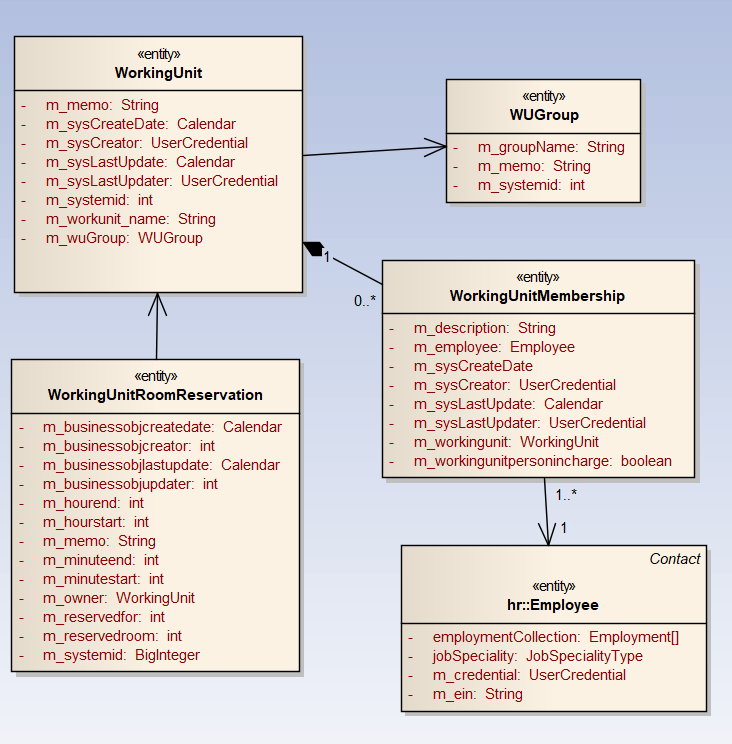
\includegraphics[width=12cm]{images/workingunit.png}}	
		\captionof{figure}{Rancangan service \textit{medical unit}}.
	\end{minipage}
\end{adjustbox}

\subsection{Perancangan Service Rawat Jalan}
Pada modul rawat jalan dibutuhkan 2 buah \textit{value object} yang membantu merepresentasikan objek \textit{customer} dan \textit{employee}. Hal ini diperlukan karena model microservice yang baru tidak menggabungkan kedua objek tersebut dalam modul rawat jalan secara langsung.\\
Berikut adalah rancangan untuk \textit{webservice} rawat jalan digambarkan menggunakan \textit{class diagram}

\begin{adjustbox}{width=1\textwidth}
	\begin{minipage}{\linewidth}
		\framebox[\textwidth]{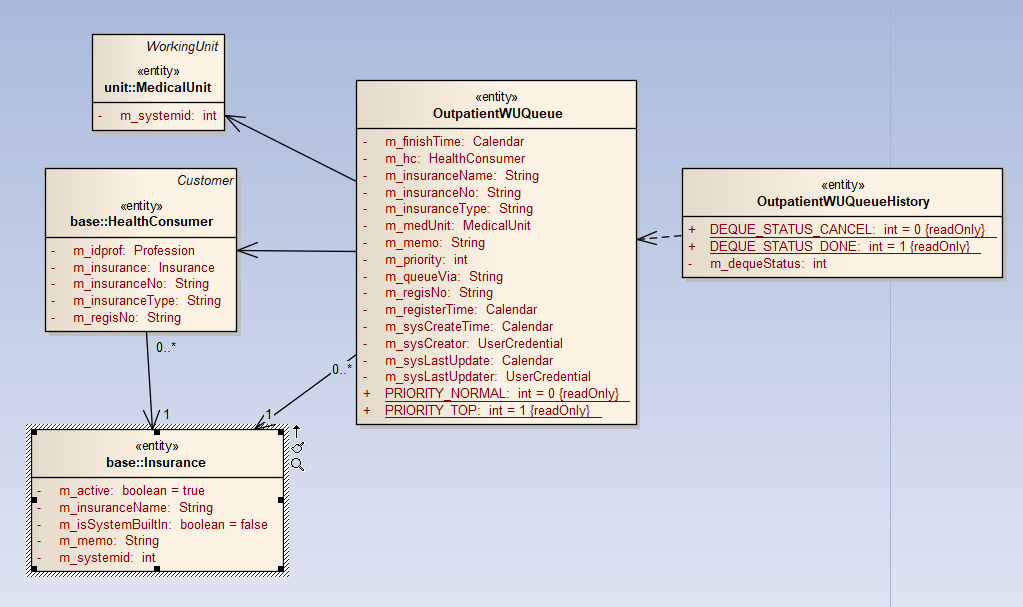
\includegraphics[width=12cm]{images/rawatjalan.png}}	
		\captionof{figure}{Rancangan service rawat jalan}.
	\end{minipage}
\end{adjustbox}

\subsection{Pemilihan Model Penyimpanan Data}
Setelah kelas-kelas service terbentuk, hal berikutnya yang harus diperhatikan adalah pemodelan manajemen data. Apabila ditinjau dari service yang dihasilkan, maka akan lebih baik menerapkan pattern database per \textit{service}, dimana satu service memiliki sebuah set database yang hanya bisa diakses oleh service tersebut dan tidak bisa saling mengakses database service yang lain.
\subsection{Pemilihan Komunikasi Antar Service}
Setelah membuat service dan database yang digunakan, hal berikutnya adalah membuat API dari service tersebut agar dapat diakses menggunakan \textit{web service}. Berdasarkan kebutuhan arsitektur microservice sendiri, model \textit{web service} yang akan digunakan adalah RESTful (\textit{Representational State Transfer}) dengan format data yang dikirim berupa JSON (\textit{JavaScript Object Notation}). Server sementara yang akan digunakan selama tahap perancangan adalah mesin pribadi milik peneliti. Setelah perancangan selesai dan siap, server baru akan dipindahkan ke server milik rumah sakit. Untuk tes pemanggilan API sementara dapat dilakukan dalam satu jaringan yang sama.
\subsection{Rancangan Deployment}
Model \textit{deployment} yang akan digunakan adalah \textit{multiple service per host}, dikarenakan lebih cocok dalam kasus penelitian yang hanya mengambill proses rawat jalan. Semua set service yang terbentuk akan di \textit{upload} dalam beberapa server agar dapat membuktikan tercapainya \textit{high availability}. Apertura sendiri memiliki 2 buah server aktif yang dapat digunakan ketika proses \textit{deployment}, serta server lainnya dapat menggunakan mesin pribadi untuk melakukan pemanggilan service dari server lain.
\section{Perbandingan Performa}
Perbandingan yang akan dilakukan adalah dengan memberikan analisa dan bukti dari bagaimana sistem bekerja pada kedua jenis arsitektur untuk setiap faktor uji yang terdiri dari : Performa, tingkat availabilitas, skalabilitas, dan reliabilitas dari sistem.
Tujuan dari test ini adalah membandingkan apakah model arsitektur microservice memberikan performa yang lebih baik apabila dibandingkan dengan arsitektur monolitik untuk kasus rawat jalan pada perangkat lunak Sistem Informasi Manajemen Rumah Sakit Apertura untuk kasus-kasus yang benar pernah terjadi dalam kurun waktu 1 tahun terakhir.

\section{Konsumer Webservice}
Konsumer adalah pihak yang melakukan pemanggilan terhadap webservice
API. Konsumer disini dibedakan berdasarkan webservice yang dipanggil. Apabila
ditinjau dari modul yang ada pada aplikasi Apertura, maka konsumer dapat
didefinisikan menjadi :
\begin{enumerate}[leftmargin=*]
	\item Konsumer dari webservice customer. Konsumer dari webservice ini bila ditinjau dari proses bisnis di gambar 3.2 adalah staff pelayanan rawat jalan	yang mendaftarkan pasien ke dalam modul rawat jalan dan staff unit medis yang akan melihat riwayat rekam medis pasien.

	\item Konsumer dari webservice medical unit. Konsumer dari webservice ini adalah staff medical unit dan juga employee itu sendiri.
	\item Konsumer dari webservice human resource. Konsumer dari webservice ini	apabila ditinjau dari proses bisnsi di gambar 3.2 adalah staff rawat jalan, staff unit medis yang berguna untuk mendaftarkan employee pada medical unit, staff rekam medis untuk menyimpan data dokter di rekam medis pasien, dan juga employee sendiri
	\item Konsumer dari webservice medical records. Konsumer dari webservice ini adalah staff unit medis yang dapat melihat rekam medis pasien dan juga staff rawat jalan.
	\item Konsumer dari webservice rawat jalan yaitu adalah staff rawat jalan sendiri yang bertugas mulai dari pendaftaran sampai proses rawat jalan itu selesai.
\end{enumerate}
\newpage